\documentclass[aspectratio=169]{beamer}
\usetheme{Madrid}
\usepackage{pgfplots}
\pgfplotsset{compat=1.18}
\begin{document}
\begin{frame}{Heights}
\begin{columns}
\begin{column}{0.4\textwidth}
\begin{itemize}
\item Left text
\end{itemize}
\end{column}
\begin{column}{0.55\textwidth}
\begin{tikzpicture}
\begin{axis}[width=\linewidth, height=0.55\textheight, xlabel={$t$}]
\addplot coordinates {(0,1) (1,0) (2,2)};
\end{axis}
\end{tikzpicture}
\end{column}
\end{columns}
\end{frame}
\begin{frame}{Paper}
\begin{tikzpicture}
\begin{axis}[width=0.4\paperwidth, height=0.3\paperheight]
\addplot coordinates {(0,0) (1,1)};
\end{axis}
\end{tikzpicture}
\begin{itemize}
\item 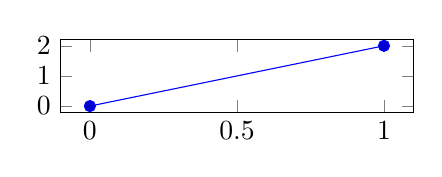
\begin{tikzpicture}\begin{axis}[width=0.5\linewidth, height=2.5cm]\addplot coordinates {(0,0) (1,2)};\end{axis}\end{tikzpicture}
\end{itemize}
\end{frame}
\end{document}
